\documentclass[mathserif]{beamer}

\mode<presentation> {
	\usetheme{PaloAlto}
	\usecolortheme{whale}
}


%\usepackage{xeCJK}
%\setCJKmainfont{WenQuanYi Micro Hei}

\usepackage{algorithm}
\usepackage{algorithmic}
\usepackage{graphicx}
\usepackage{booktabs}
\usepackage{fontspec}
\usepackage{xunicode}
\usepackage{xltxtra}

\usepackage{amsmath,amssymb}

\setbeamercovered{transparent}
\logo{
\includegraphics[height=1.58cm]{./logo.jpg}}

%----------------------------------------------------------
%	Title Page
%----------------------------------------------------------

\title[Finding TPMFP in BTD]{Finding Time Period-Based Most Frequent Path in Big Trajectory Data\thanks{powered by \XeLaTeX} }

\author{Ziyang Chen}
\institute[FDU]
{
	Fudan University\\
	\medskip
	\textit{13307130148@fudan.edu.cn}
}
\date{\today}

\begin{document}
\newtheorem{property}[theorem]{\textsc{Property}}
\newtheorem{defination}[theorem]{\textsc{Defination}}
\newtheorem{theore}[theorem]{\textsc{Theorem}}
\newtheorem{lemm}[theorem]{\textsc{Lemma}}

\begin{frame}
\titlepage
\end{frame}

\AtBeginSection{
	\begin{frame}
	\frametitle{Summary}
	\tableofcontents[currentsection, hideothersubsections]
	\end{frame}
}

\section{Overview}
\begin{frame}{Overview}
	\begin{itemize}
	\item The main task: find \textit{the most frequent}(MFP) during user-specified time periods in large-scale historical trajectory data.
	\item They refer to this query as \textit{time period-based MFP}(TPMFP).
	\item Specifically, given a time peroid $T$, a source $v_s$ and a destination $v_d$, TPMFP searchs the MFP from $v_s$ to $v_d$ during $T$.
	\end{itemize}
\end{frame}

\begin{frame}{Overview}
	\begin{itemize}
	\item None of the previous work can well reflect people's common sense notion which can be described by the following key properties:\\
		\begin{itemize}
		\item \textit{suffix-optimal}
		\item \textit{length-insensitive}
		\item \textit{bottleneck-free}
		\end{itemize}
	\item The first task is to give a TPMFP definition that satisfies the above three properties.
	\item The next task is to find TPMFP over huge amount of trajectory data efficiently.(over $11,000,000$ trajectories.)
	\end{itemize}
\end{frame}

\section{Properities}
\begin{frame}{Key Properities}
	\begin{property}[\textsc{Suffix-Optimal}]
	Let $P^*$ denote the $v_s-v_d$ MFP. For any vertex $u \in P^*$ , the sub-path (suffix) of $P^*$ from $u$ to $v_d$ should be the $u–v_d$ MFP.
	\end{property}
	\begin{property}[\textsc{Length-Insensitive}]
	The length of any path should not be a deciding factor of whether it is the $v_s-v_d$ MFP.
	\end{property}
	\begin{property}[\textsc{Bottleneck-Free}]
	The MFP $P^*$ should not contain infrequent edges(i.e., bottlenecks).
	\end{property}
\end{frame}

\section{Definations}
\begin{frame}{Definations}
\begin{defination}[\textsc{Road Network}]
A road network is a directed graph $G = (V, E)$ where $V$ is a set of vertices representing road intersections and $E$ is a set of edges representing road segments.
\end{defination}
\begin{defination}[\textsc{Path}]
Given $G$, an $x_1–x_k$ path is a non-empty graph $P = (V_p, E_p)$ of the form $Vp = {x_1, x_2,\ldots{}, x_k}$ and $E_p = {(x_1, x_2),\ldots , (x_{k−1}, x_k)}$ such that $P$ is a sub-graph of $G$ and the $x_i$ are all distinct.
\end{defination}
\begin{defination}[\textsc{Trajectory}]
Given $G$, a trajectory $Y$ is a sequence $((x_1, t_1), (x_2, t_2), \ldots , (x_k, t_k))$ such that there exists a path $x_1 \to{} x_2,\to{},\dots,\to{} x_k$ on $G$ and $t_i$ is a timestamp indicating the time when $Y$ passes $x_i$.
\end{defination}
\end{frame}

\begin{frame}{Definations}
\begin{defination}[\textsc{Footmark}]
Given $\Omega{} = (G, \Upsilon{}, v_s,v_d,T)$ and a trajectory $Y = ((x_1, t_1), \ldots{} , (x_k, t_k)) \in{} \Upsilon{}$, if there exists a non-empty sub-trajectory $Y'$ of $Y$ from $Y[i]$ to $Y[j]$ such that:\
	\begin{itemize}
		\item $Y'.d = v_d, i.e., Y'[j].v=v_d,$
		\item $[Y'.t_s,Y'.t_e]\subseteq{} T,i.e.,[Y[i].t,Y[j].t]\subseteq{} T,$
		\item $Y[i−1].t\notin{} T$,if $i>1$,
	\end{itemize}
	then path $Y'.P$ is the footmark of $Y$ w.r.t. $v_d$ and $T$ , denoted as $\widetilde{Y}􏰀 (v_d ,T)$.
\end{defination}
\end{frame}

\begin{frame}{Definations}
\begin{figure}
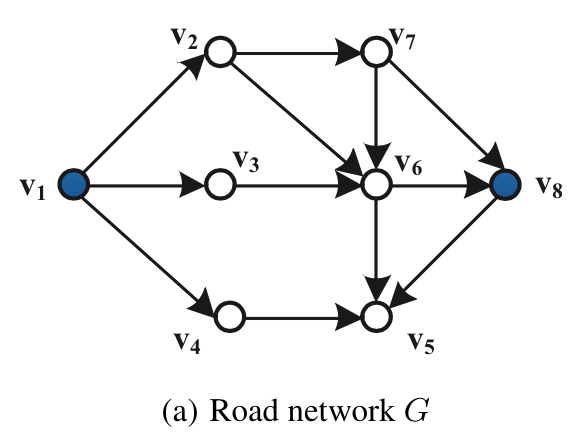
\includegraphics[width=4cm]{pic1.png}
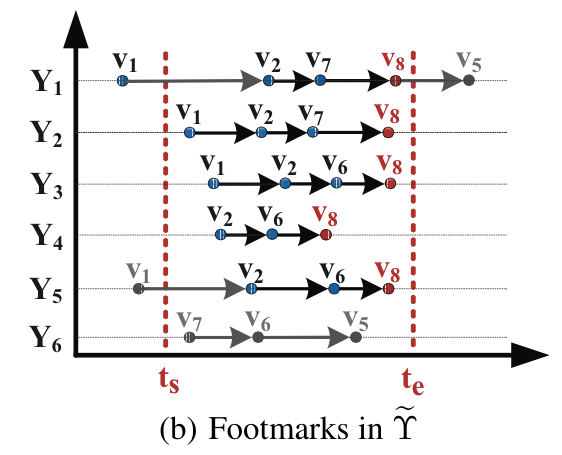
\includegraphics[width=4cm]{pic2.png}
\end{figure}
\begin{figure}
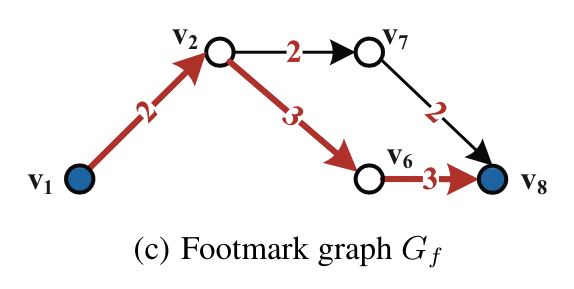
\includegraphics[width=5cm]{pic3.png}
\end{figure}
\end{frame}

\begin{frame}{Definations}

\begin{defination}[\textsc{Edge Frequency}]
Given $G$, $\widetilde{\Upsilon}_{(v_d,T )}$, and an edge $(u, v) \in{} G$, the edge frequency $F (u, v)$ is the number of the footmarks in $\widetilde{\Upsilon}_{(v_d,T )}$ containing$(u,v)$.
\end{defination}
\begin{defination}[\textsc{Footmark Graph}]
Given $G$ and $\widetilde{\Upsilon}_{(v_d,T )}$, a footmark graph $G_f$ is a weighted sub-graph of $G$ such that:
	\begin{itemize}
	\item for any edge $(u,v) \in G$, $w_{uv} = F(u,v)$;
	\item edge $(u,v)\in{}G_f$, if and only if $(u,v)\in{} G $and $w_{uv}>0 $.
	\end{itemize}
\end{defination}
\end{frame}

\begin{frame}{Definations}
\begin{defination}[\textsc{Path Frequency}]
Given $G_f$ , the frequency of path $P (to \; v_d)$ is a sequence $F(P) = (f_1,...,f_k)$ where:
	\begin{itemize}
	\item $\{f_i|i \in{} {1,\ldots{},k}\} = \{w_{uv}|(u,v) \in{} E(P)\}$,
	\item $f_1 \leq{} f_2 \leq{} \ldots{} \leq{} f_k$.
	\end{itemize}
\end{defination}
\end{frame}

\begin{frame}{Definations}
\begin{defination}[\textsc{More-Frequent-Than Relation}]
Given two path frequencies $F(P) = (f_1,\dots{},f_m)$ and $F(P') = (f_1',\ldots{},f_n' )$ w.r.t. the same $G_f$ , $F (P )$ is more-frequent-than $F (P')$, denoted as
$F (P ) \succeq{} F (P' )$, if one of the following statements holds:
	\begin{itemize}
	\item $F(P)$ is a prefix of $F(P')$;
	\item there exists a $q \in{} \{1,\ldots{},min(m,n)\}$ such that 1) $f_i = f_i'$
for all $i \in{}\{1,\ldots{},q−1\}$, if $q>1$, and 2) $f_q >f_q'$.
	\end{itemize}
Particularly, $F(P)$ is strictly-more-frequent-than $F(P')$, denoted
as $F(P) \succ{} F(P')$, if $F(P) \succeq{} F(P')$ and $F(P) \neq{} F(P')$.
\end{defination}

\end{frame}

\begin{frame}{Problem Statement}
\begin{theore}
The more-frequent-than relation is a total order.
\end{theore}
\begin{defination}[MPF]
Given $G_f$ and a $v_s–v_d$ path $P_* \subseteq{} G_f$, if $F(P_*) \succeq{} F(P)$ holds for every $v_s–v_d$ path $P \subseteq{} G_f$, then $P_*$ is the $v_s–v_d$ MFP w.r.t. $G_f$.
\end{defination}
\textbf{Problem Statement:} Given $\Omega{} = (G, \Upsilon{}, v_s, v_d, T )$ where $\Upsilon{}$ is a very large set of historical trajectories, we need to find the TPMFP which is the MFP w.r.t. $G_f$ . Note that $G_f$ is the footmark graph derived from $\Omega$.
\end{frame}

\section{Alogrithm}
\subsection{Overview Algorithm}

\begin{frame}{Overview Algorithm}
\begin{figure}
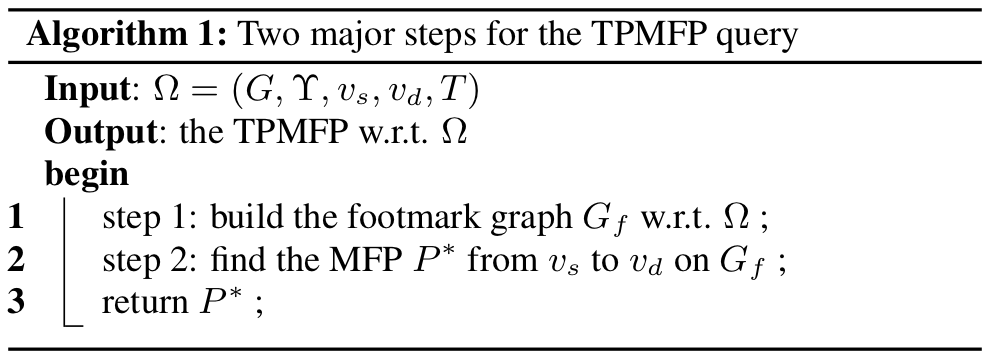
\includegraphics[width = 10cm]{alg1.png}
\end{figure}
\begin{theore}
Given $\Omega{} = (G, \Upsilon{}, v_s, v_d, T )$, let $P_*$ be the $v_s–v_d$ TPMFP w.r.t. $\Omega$. Then, for every vertex $u \in{} V (P )$, the sub-path of $P_*$ from $u$ to $v_d$ is the $u–v_d$ TPMFP.
\end{theore}
\end{frame}

\subsection[FMI]{Footmark Index}
\begin{frame}{Footmark Index}
They design an index called Footmark Index (FMI):
\begin{itemize}
\item Build a $B^+ - tree \; BT_{v_i}$ for each vertex $v_i \in{} V (G)$
\item $BT_{v_i}$ indexes the time of the trajectories reaching $v_i$ and stores the corresponding trajectory id’s
\item Each leaf entry of $BT_{v_i}$ is of the form $<tid,t_a>$
\item Given $v_d$ and T , FMI-Search$(v_d , T )$ returns the id’s of all the trajectories in $\Upsilon{}(v_d,T )$ via searching $BT_{v_d}$
\end{itemize}
\end{frame}

\begin{frame}{Footmark Index}
\begin{figure}
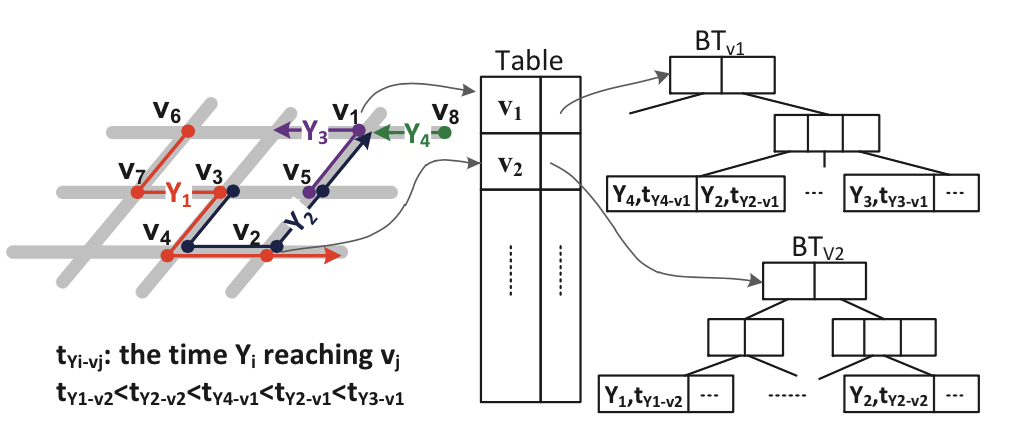
\includegraphics[width = 10cm]{FMI.png}
\end{figure}
\end{frame}

\begin{frame}{Footmark Index}
\begin{figure}
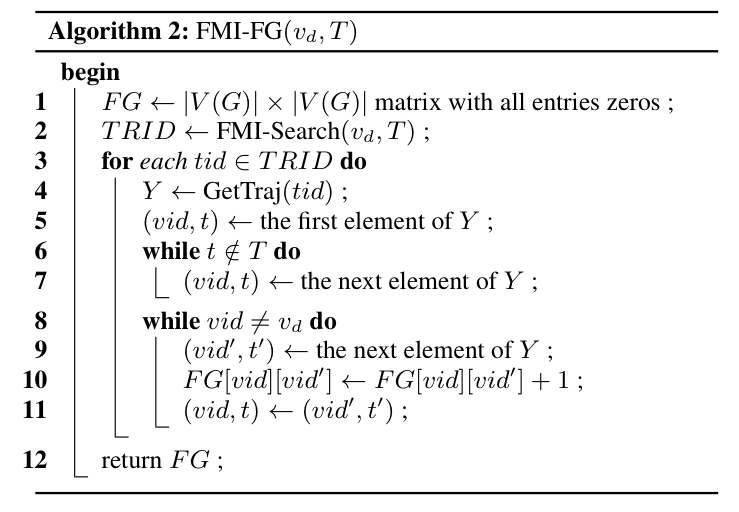
\includegraphics[width = 10cm]{alg2.png}
\end{figure}
\end{frame}

\subsection[CMFI]{Containment-Based Footmark Index}
\begin{frame}{Containment-Based Footmark Index}
	\begin{itemize}
	\item FMI incurs $|\Upsilon(v_d,T)|$ page accesses
	\item Organizing the involved trajectories into different groups
	\item In each group, the front part of each trajectory Y before reaching $v_d$ (including $v_d$), denoted as $Y_{*–v_d}$ , is 'contained' by a unique 'dominant' trajectory
	\item Only need to fetch the 'dominant' trajectory
	\item They refer to this new index as Containment-Based Footmark Index (CFMI)
	\end{itemize}
\end{frame}

\begin{frame}{Containment-Based Footmark Index}
\begin{defination}[$v_d$-\textsc{Containment}]
For two trajectories $Y$ and $Y'$ in $\Upsilon{}_{v_d}$ , if $Y_{*–v_d}.P$ is a sub-path of $Y'_{*-v_d}.P$, then $Y$ is $v_d$-contained by $Y'$. In particular, if $Y_{*–v_d}.P \neq{} Y'_{*-v_d}.P $, then $Y$ is stickly $v-d$-contained by $Y'$.
\end{defination}
\begin{defination}[$v_d$-\textsc{Dominant}]
A trajectory $Y \in{} \Upsilon{}_{v_d}$ is $v_d$-dominant if there exists no $Y' \in{} Υ_{v_d}$ such that $Y$ is strictly $v_d$-contained by $Y'$.
\end{defination}
\end{frame}

\begin{frame}{Containment-Based Footmark Index}
	\begin{itemize}
	\item CFMI improves the structure of each $B^+-tree$ in FMI. Specifically, each leaf entry of $BT_{v_i}$ is in the following new form: $<tid,t_s,t_a,did,sloc>$
	\item Besides, we keep a table $v_i-Dom$ for each $BT_{v_i}$ , in which we record the length of $Y_{*–v_i}.P$ for each $v_i$-dominant trajectory $Y$
	\end{itemize}
\end{frame}

\begin{frame}{Containment-Based Footmark Index}
	For each query $(v_i, T)$, CFMI returns two sets:
		\begin{enumerate}
		\item $TRREC =\{(tid, t_s , did, sloc)\}$, which records the information of trajectories in $\Upsilon{}(v_d ,T )$
		\item $DOM = \{(did, len)\}$, which records the did’s appeared in TRREC and their corresponding values in $v_i - Dom$ 
		\end{enumerate}
\end{frame}

\begin{frame}{Containment-Based Footmark Index}
\begin{figure}
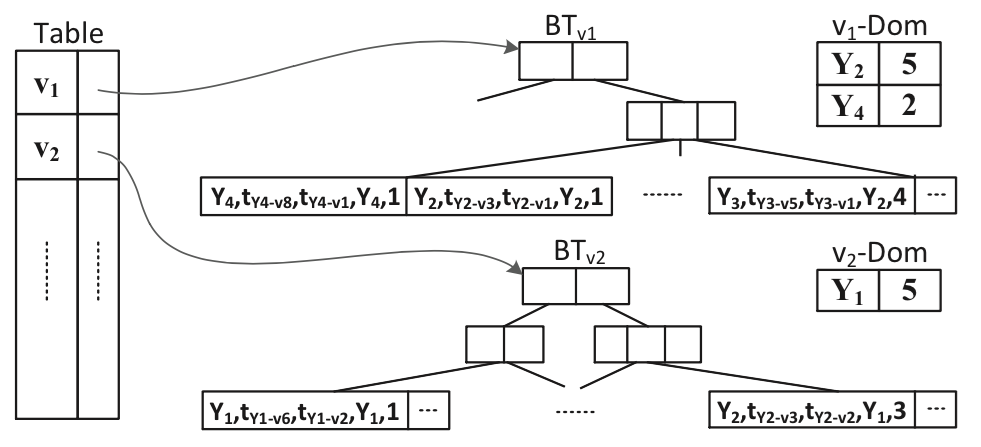
\includegraphics[width = 10cm]{CFMI.png}
\end{figure}
\end{frame}

\begin{frame}{Containment-Based Footmark Index}
\begin{figure}
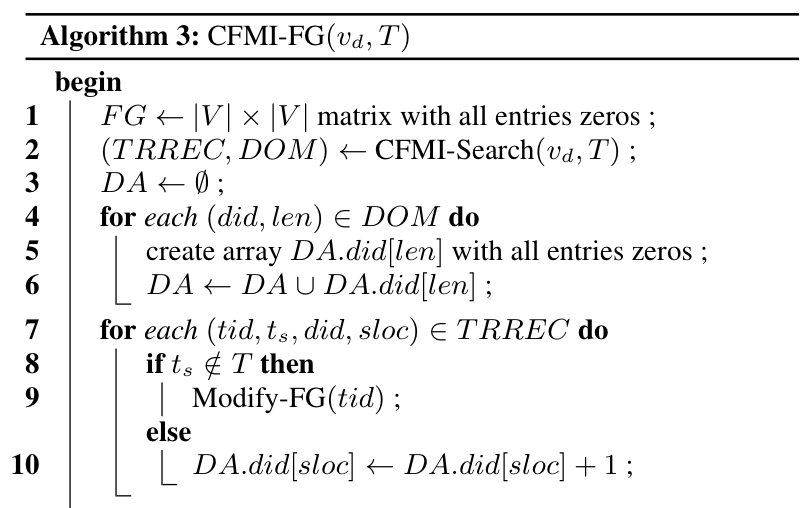
\includegraphics[width = 10cm]{alg3_1.png}
\end{figure}
\end{frame}

\begin{frame}{Containment-Based Footmark Index}
\begin{figure}
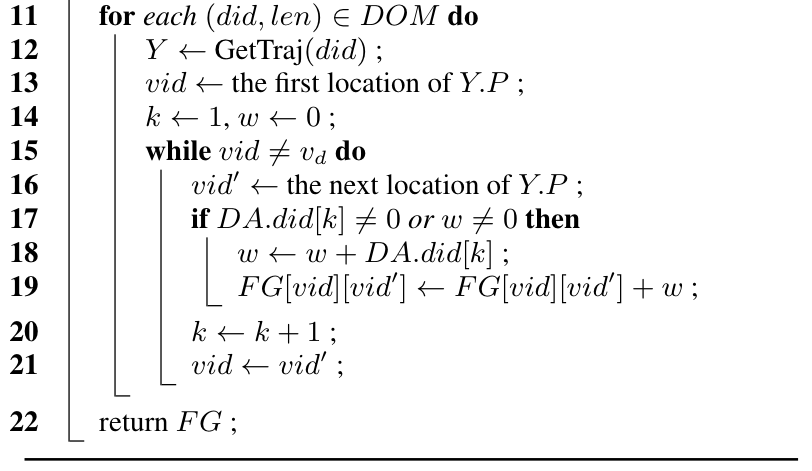
\includegraphics[width = 10cm]{alg3_2.png}
\end{figure}
\end{frame}

\subsection{MFP-Search}

\begin{frame}{MFP-Search}
\begin{lemm}
Let $u \leadsto{} v$ denote a path from u to v. Suppose $P^c =v_s \leadsto{} 􏰁v_k \leadsto{} v_k \leadsto{} 􏰁v_d$ is a path with cycles on $G_f$. We have $F (P ) \succ{} F (P^c )$, where $P$ is the resulting path after removing the portion of $P^c$ between consecutive visits to $v_k$.
\end{lemm}
\begin{lemm}
Given $G_f$ w.r.t. $\Omega{}$, there exists an MFP from $v_s$ to $v_d$ that is simple, i.e., has at most $|V_f| − 1$ edges.
\end{lemm}
\end{frame}

\begin{frame}{MFP-Search}
Define '+' as follows:
\begin{itemize}
\item If the two inputs are non-decreasing sequences of positive integers, "+" merges them into a non-decreasing sequence. For example: $(20) + (5, 20) = (5, 20, 20)$;
\item If one input is $\emptyset{}$, then the other input is returned. If both inputs are $\emptyset{}$’s, then $\emptyset{}$ is returned. For example: $\emptyset{} + (5, 20) = (5, 20)$;
\item If one input is $\#$, then $\#$ is returned. For example: $\# + (5, 20) = \#$.
\end{itemize}
\end{frame}

\begin{frame}{MFP-Search}
Let $F^*(v_s, i)$ be the frequency of the $v_s–v_d$ MFP\\ using at most i edges.
\begin{lemm}
Given $G_f = (V_f,E_f)$, if $i > 0$, then we have
\begin{displaymath}
F^*(v_s,i) = \max(F^*(v_s,i−1), \max_{(v_s,v) \in{} E_f} ((w_{v_sv})+F^*(v,i−1))).
\end{displaymath}
\end{lemm}
\end{frame}

\begin{frame}{MFP-Search}
\begin{figure}
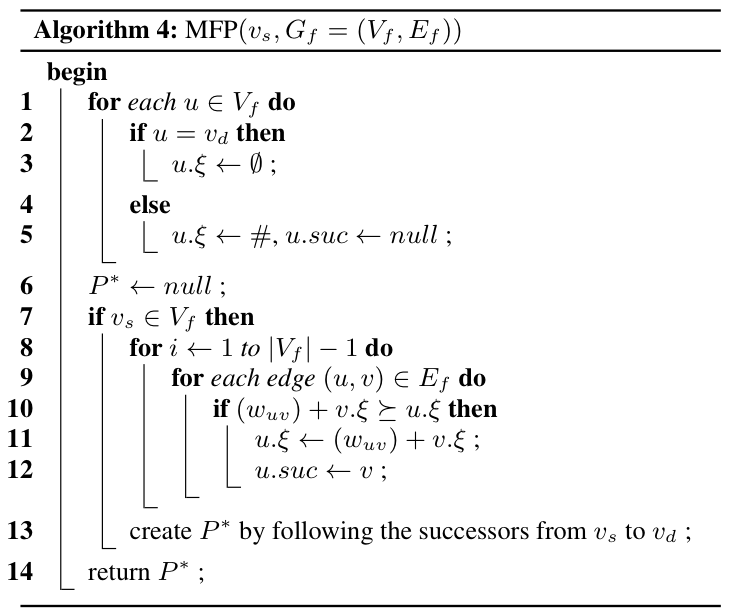
\includegraphics[width = 8cm]{alg4.png}
\end{figure}
\end{frame}

\section{Experiment}

\subsection[D\&{}E]{Dataset \&{} Environment}
\begin{frame}{Dataset \&{} Environment}
\begin{block}{Dataset}
\begin{small}
\begin{tabular}{|l|r|r|r|}
\hline
Dataset Name & No. of Trajectories & Total Length & Size (MB)\\
\hline
Year Dataset & 11,547,611 & 245,276,717 & 3,335\\
\hline
Month Dataset & 1,650,134 & 35,619,454 & 484\\
\hline
Day Dataset & 54,579 & 1,217,890 & 17\\
\hline
\end{tabular}
\end{small}
\end{block}


\begin{block}{Environment}
\begin{small}
\begin{itemize}
\item Intel(R) Xeon(R) E5506 CPU (2.13GHz)
\item 12GB memory
\item 10,000RPM sever-level hard disks
\item Linux 2.6.32 x86\_64
\item Jre 1.7.0\_4 64-Bit
\end{itemize}
\end{small}
\end{block}
\end{frame}


\subsection{Effectiveness}
\begin{frame}{Effectiveness}
\begin{figure}
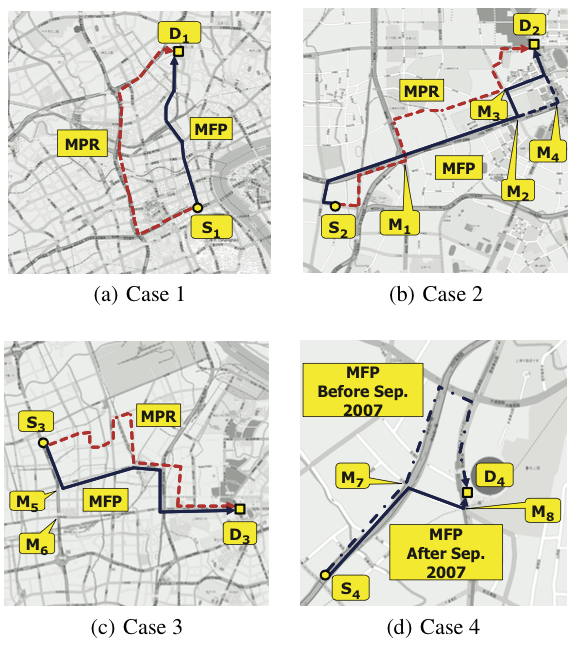
\includegraphics[width = 6cm]{exp1.png}
\end{figure}
\end{frame}

\begin{frame}{Effectiveness}
\begin{figure}
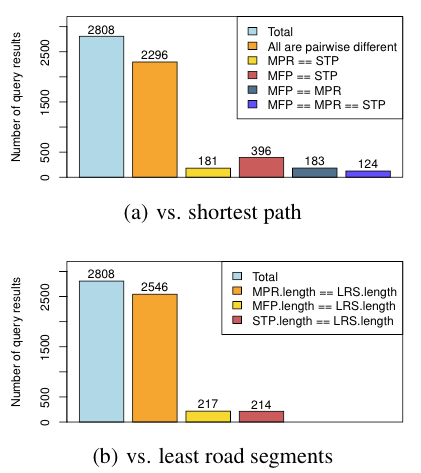
\includegraphics[width = 6cm]{exp2.png}
\end{figure}
\end{frame}

\subsection{Effciency}

\begin{frame}{Index Creation and Size}
\begin{block}{Index Creation}
For Year Dataset, the index creation time of FMI and CFMI is 72 minutes and 127 minutes, respectively.\\
\end{block}

\begin{block}{Index Size}
\begin{figure}
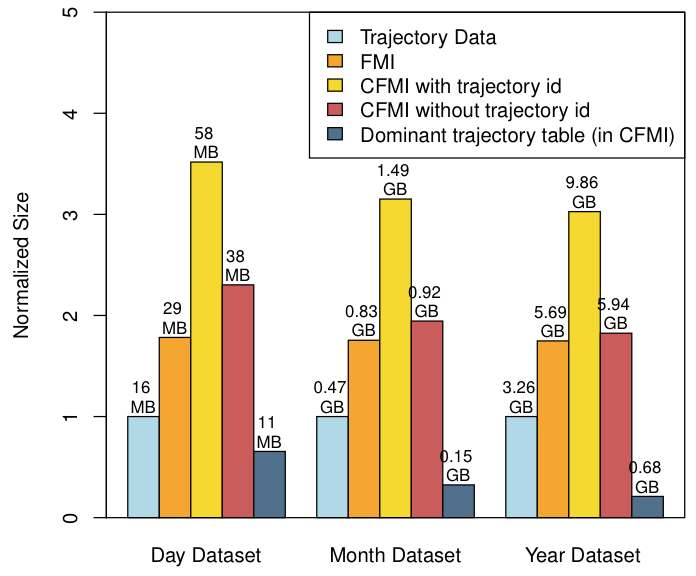
\includegraphics[width = 5cm]{exp3.png}
\end{figure}
\end{block}
\end{frame}

\begin{frame}{Effciency of MFP-Search}
\begin{figure}
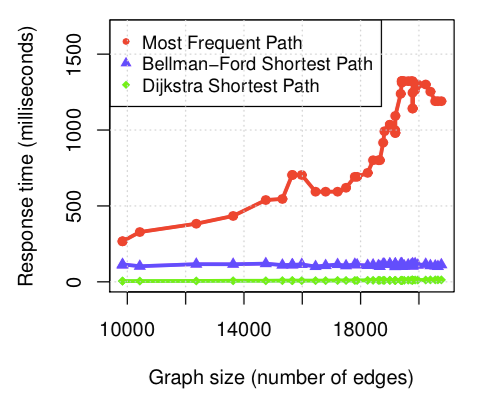
\includegraphics[width = 7cm]{exp4.png}
\end{figure}
\end{frame}

\begin{frame}{Effciency}
\begin{figure}
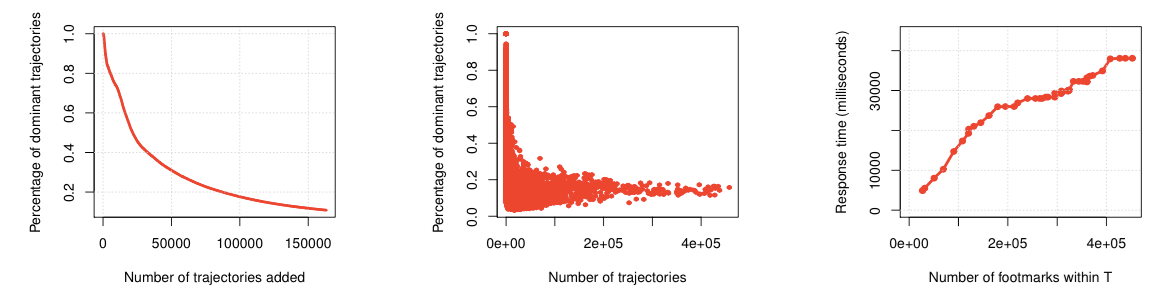
\includegraphics[width = 10cm]{exp5.png}
\end{figure}
\begin{figure}
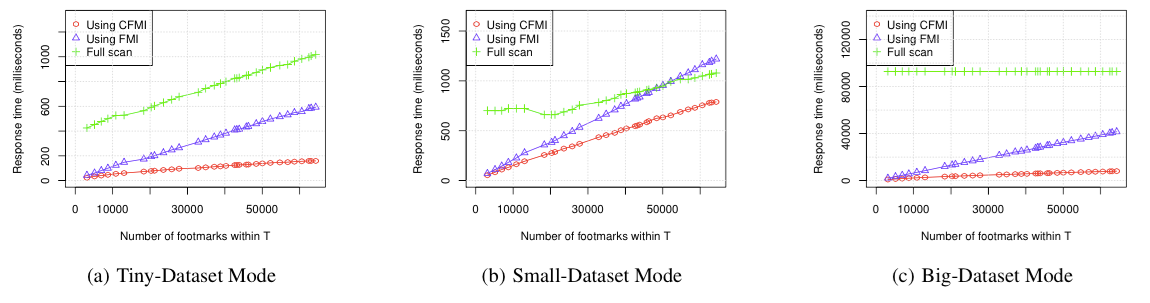
\includegraphics[width = 10cm]{exp6.png}
\end{figure}
\end{frame}

\AtBeginSection{}

\section[Q\&{}A]{}
\begin{frame}{Q\&{}A}
  \color{blue}\huge{Any Questions?}
\end{frame}

\section[End]{}
\begin{frame}{End}
  \color{blue}\huge{Thanks For Attention!}
\end{frame}

\end{document}
